% $Id$

%\section{Object Model}

The following section describes design considerations for
Fields and FieldBundles, and the relationship between and subdivison of
responsibilities into separate objects.
It also discusses ESMF Arrays and DataMaps and their
role in supporting the storage and movement of user data.
This section of the document discusses the design using 
Object Oriented terminology which most directly maps 
to a C++ implementation, but by using selected
capabilities of Fortran 90/95 (e.g. interface blocks,
derived types, etc.) the same concepts can be implemented.
See the ESMF Implementation Report~\ref{implrep} for more details.

\subsection{Fields}

A Field object consists of two major internal subobjects: a GlobalField object
and a LocalField object.  This separation allows the code to clearly
differentiate between functions which operate internal to a single DE
on a local decomposition of data, 
and those which access the global state of the Field.  
 
There is a correspondence between the Global Distributed Grid object,
and the Local Distributed Grid object, and Fields.  Each DE contains
the corresponding local decompositions for Distributed Grids and Fields.

Field objects maintain the relative location, or relationship, of
how data maps onto the grid (e.g. one item per cell located at
the cell center, one item per cell located at the NW corner, 
one item per cell vertex, etc).  Different Fields
which are on the same underlying Grid but have different
relative locations
can share the same Grid object without
needing to copy or replicate it multiple times.  Regridding
operations can operate first on the shared Grid, and then
use the relative location information from the Field to compute the
corresponding transformation of the data.

Some methods which have a Field interface will actually be
implemented at the underlying Grid or Array level; they
will be inherited by the Field object.  This allows the user
API (Application Programming Interface) to present functions at
the level which is most consistent to the application without
restricting where inside the ESMF the actual implementation
is done.

\subsection{FieldBundles}

FieldBundles depend on the underlying Fields for most of their 
communication and querying functions.  The information which
must be maintained in the FieldBundle object is a list of constituent
Fields, and whether there is a packed Array at the FieldBundle level.

Memory layout information is encapsulated in an DataMap object which
is attached to the Array.  It can be accessed by the FieldBundle
by querying the Array.

The FieldBundle object collects multiple Field objects which share a
common or compatible Grid object.  In addition to the basic methods for
setting, retrieving, and querying the constituent Fields, it provides
methods for configuring and querying memory layouts for the Array
and some limited collective operations on all Fields in a FieldBundle.

\subsection{Array}

An ESMF Array object is a small amount of description about
the data (metadata, or "dope vector" in Fortran terminology), 
plus the data buffer itself.  It is 
responsible for maintaining
information about the individual value type (e.g. float, integer), 
the physical representation (e.g. Cray format float vs IEEE), 
data count, and memory ordering information when multidimensional
arrays are linearized in memory.
The metadata is stored in an ArraySpec
derived type/structure (see below).

Fields maintain the status of who ``owns'' the local data;
the DataDetach method is called at the Field level and it
returns the data contained in the Array class.
After the DataDetach routine is called, responsibility for
the data array is now with the calling code which can iterate through
and update data values freely.  Before allowing calls to methods which need
access to the data, such as Regridding, Halo updates, and
data exchange during Coupling, the Field must ensure that it
has regained ownership of the data via a DataAttach call.  
This ensures that data values are not being updated by one
DE at the same time another DE is trying to read out a consistent
set of data values.


The DataMap objects maintain mapping information between the
Grid and the ESMF Array objects contained in a Field object.
This includes how the indices map, what the unit data values are,
the RelativeLocations of the data items to a single Grid element
(this is related to but separate from the Grid "staggering" value).
It also contains interleaving information for vectors and for
packed Data associated with a FieldBundle.
Vector data which must be transformed if the underlying grid
is transformed (e.g. u,v wind vectors) must be tagged as such
so the framework can transform the data and maintain consistency
if the grid is rotated or transposed.

\subsubsection{Indexorder}

The index order specification is 
a simple derived type in Fortran and a structure in C++.
It contains the ordering of how the indices in a multidimensional
array vary from inner to outer (fastest to slowest in iteration
order).  Grid and Array objects use this.

\subsubsection{Interleave}

The interleave specification is a 
derived type in Fortran and a structure in C++.
It contains the ordering of how items with more than
a single element (e.g. a 3-vector) are organized; 
interleaved (x1,y1,z1), (x2,y2,z2) or 
block (x1,x2,x3...) (y1,y2,y3,...) ...
DataMap objects use this.

%\subsection{Objects with direct relationships}

Figures~\ref{fig:fieldhier} and \ref{fig:bundlehier} show the object hierarchy of
%those objects which are subobjects or aggregated objects
%of Fields and FieldBundles.

\begin{figure}
\caption[Field hierarchy]{The object hierarchy for objects closely related to Fields.}
\label{fig:fieldhier}
\scalebox{0.70}{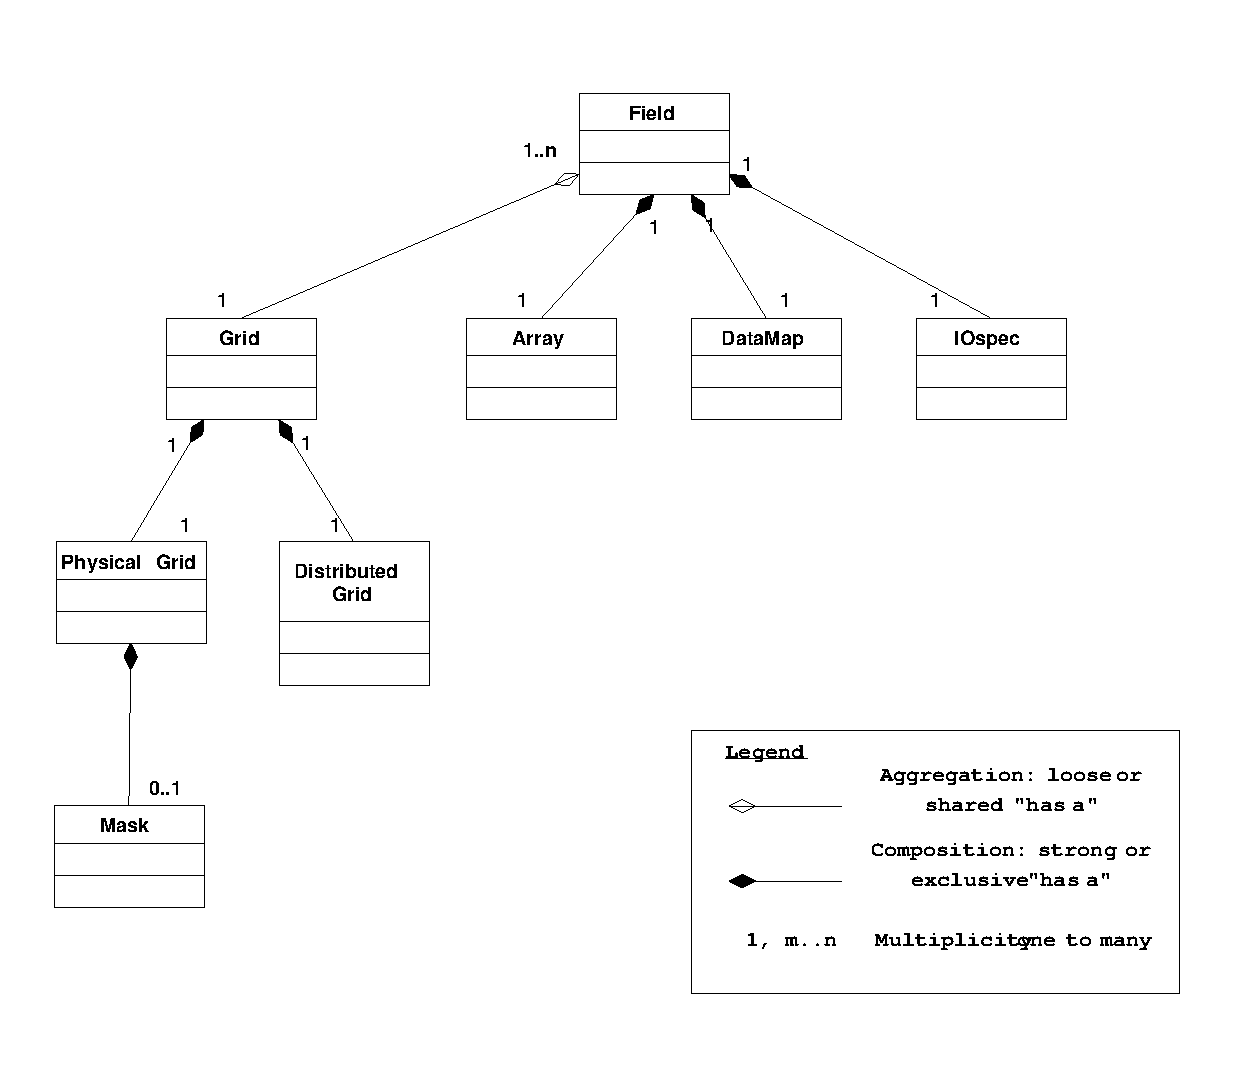
\includegraphics{fieldclassNH.eps}}
\end{figure}

%\begin{figure}
%\caption[FieldBundle hierarchy]{The object hierarchy for objects closely related to FieldBundles.}
%\label{fig:bundlehier}
%\scalebox{0.70}{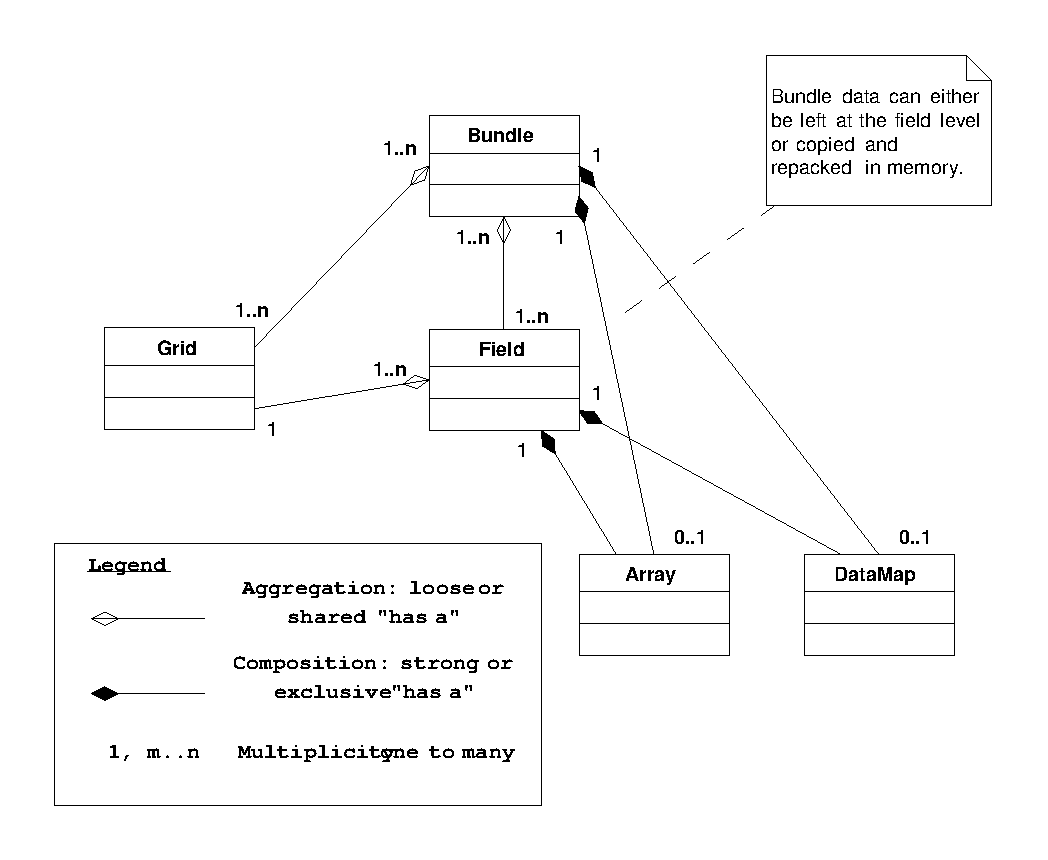
\includegraphics{bundleclassNH.eps}}
%\end{figure}

A more detailed description of the interactions between
these objects and Fields and FieldBundles follows.

\subsubsection{Grids}

A Grid object is responsible for
maintaining all information about the global coordinates and about how
the decomposition of the whole problem is spread across multiple
processing elements.  
See Section~\ref{<<FIXME>>} for more information about Grid objects.  
The Field object uses information from the Grid object to provide
two different types of views of the Field to the calling code.
One is a unified logical view of the entire Field as a whole
regardless of the current decomposition.  The other view allows code
running on a single processing element to query and retrieve a pointer 
to the subset of the Field which is local to that processing element,
and to make requests that result in data being updated among neighboring
subsets (e.g. Halo updates).

A PhysicalGrid is sometimes an algorithmic description of the
grid coordinates and does not need to be stored locally.  But if
the PhysicalGrid is unstructured, or if it must be explicitly
listed then it can be up to as large as the data arrays and
must be partitioned just as the data is and stored locally per PE.
In this case, there is a Global part and a Local part to the PhysGrid
object.

A Field must contain a Grid object to be valid even if the data does not
have any spatial location.  This is to allow subsetting across multiple
processors and to ensure that Validation routines can distinguish between
Fields with no coordinate information and invalid Field objects.

\subsubsection{Mask}

A Mask object maintains information about which data items are
valid, for example land gridpoints which are invalid in an ocean model.
The Mask object may store the valid/invalid list in the most 
compact internal representation available, but has methods to
retrieve the information in either an explicit point list of
valid or invalid points, or a 1-for-1 array which matches the
data array length, each entry being a 0/1 flag to indicate validity.
A Mask object may also contain categories of valid or invalid points, 
for example 1=Pacific, 2=Atlantic, etc.

\subsubsection{IOSpec}

The ESMF will attempt to encapsulate 
all differences between I/O to various file formats
under the I/O subsystem layer.  However, there are
several things the user will want to select when
doing file I/O, such as the file in which various
Field data will be found, etc.  For those file formats
with metadata, there may be a description of the data
which can be read by the ESMF and need not be
specified by the user, but for metadata-poor formats,
things like data type, size, shape, etc may have to
be specified.

\subsection{Objects with more distant relationships}

\subsubsection{Regrid}

A Regrid object does a transformation of data, either from
one Grid to another, or within the same grid but with some remapping
or transformation of the data values.  The input objects to
some of the Regridding functions will be Fields because they
hold the connection between the Grid object and the corresponding
data fields.  The Regrid methods can detach the data, determine
the mapping from the old Grid to new Grid, alter the data, and
create a new Field with the transformed data.

\subsubsection{Subset}

A Subset object 
exists to encapsulate the possible types of subsetting an existing
Field or FieldBundle.  This might include subsetting by Bounding Box,
by Hyperslab, by strides through the data, and other options.
The use of Subset objects simplifies the interface to
any operations which allow subsetting, by separating the
possibly complicated specification of the subset from the
actual use.  The Subset methods will know how to operate on Field
objects to create new Fields and Grids.

\subsubsection{Registry}

The Registry object contains methods used in name management
as well as global (name, value) configuration information.
The name management is a general dictionary utility.  It
manages multiple namespaces (e.g. per application, per component,
per field, per grid, etc) and contains methods used by the
Field and FieldBundle objects to ensure Field and FieldBundle names
are unique, and to generate unique names if the caller does
not specify a field name.
% examples of methods i can see fields using:
% Does Name Exist?
% List NameSpaces
% List Names within a Space - this implies broadcast
%   if space exists across more than a single DE (process)
% Generate Unique Name
% Add Name provided its unique
% seems like names should in general be (name,id) so
% subsequent requests can be id based.  or use id for
% a handle and the ids uniquely identify the name and
% or namespace.
The configuration management methods include those to 
read in (name, value) pairs from a config file, and to query
and return this information, for example to discover the
filename associated with a particular field name and
any directives on I/O options.


\subsubsection{Log}

A Log object contains methods used to write debugging, status,
and error information to a log file.

\subsubsection{Base object}

The Attribute object can be associated with any object in the system,
and maintains a list of (name,value) pairs.  Fields are required to
have at least a unique name, so all Field objects will have an associated
Attribute object.

